\section{SuffixDecoding}
\label{sec:suffix-decoding}

The goal of \emph{SuffixDecoding} is to enable fast, adaptive speculative decoding over long sequences, particularly suited for agentic applications where repeated inference calls often contain highly predictable and overlapping token sequences. In such settings, long stretches of output can be accurately predicted from prior and ongoing requests.

To fully exploit these opportunities, SuffixDecoding must address two key challenges. First, it must support \emph{fast generation of speculative sequences}—including long continuations---without relying on draft models or expensive token-by-token prediction. Second, it must be \emph{adaptive} to the current prediction context: aggressively speculating long continuations only when they are likely to be accepted, and speculating shorter sequences when uncertain to avoid wasted verification compute.

To support fast speculation, SuffixDecoding builds a \emph{suffix tree}~\citep{10.1109/SWAT.1973.13} over the tokens in the current and prior requests, and uses the suffix tree to generate speculative tokens.
The root node of the tree represents the beginning of a suffix of any token sequence stored in the tree, each child of a node represents a specific token which is a possible continuation from its that node, and the path from the root to each node represents a distinct subsequence.

For each request, we consider speculating token sequences from (1) the prompt and output of that request, and (2) the outputs of prior requests. Doing so captures the source of output token repetition from many agentic algorithms, including self-consistency, self-refinement, and multi-agent pipelines.

SuffixDecoding leverages suffix trees to perform fast pattern matching and find possible continuations of token sequences. Suppose the prompt and output tokens of an ongoing inference is \( x_{1:t} \). Consider a suffix \( x_{t-p+1:t} \) of length \( p \), which we will refer to as the \emph{pattern} sequence. We walk the suffix tree starting from the root node, and at each step taking the child that corresponds to token \( x_{t-p+i} \). If no such child exists, then the pattern is not found and SuffixDecoding reverts to standard non-speculative decoding. Otherwise, after \( p \) steps, we arrive at a node whose descending paths are the possible continuations of the pattern sequence.

Although this procedure can quickly find a (potentially large) set of candidate sequences, verifying all of them in speculative decoding may be cost-prohibitive. Instead, SuffixDecoding builds a much smaller and more likely speculation tree through a greedy expansion and scoring procedure, and uses this smaller tree in tree-based speculation. An overall illustration of SuffixDecoding is shown in Fig.~\ref{fig:suffix-decoding}, which we detail in the rest of this section.

\paragraph{Suffix Tree Construction.}

Building the suffix tree and updating it as part of an online inference service involves two stages. First, the previous inference outputs can be added to the tree in a single offline processing step (e.g. from historical logs), or online during inference serving after each inference request completes. Second, the current ongoing prompt and out tokens are added online as new requests are received and as each new token is generated.

In reality, we found it convenient to maintain two different suffix trees: a \emph{global} tree for the previously generated outputs, and a separate \emph{per-request} tree for the current ongoing inference request. This circumvents the complexities and overheads due to synchronizing the suffix tree updates from multiple concurrent requests. The global tree can be constructed offline in \( O(n) \) time, while the per-request tree can be efficiently constructed and updated online~\citep{10.1007/BF01206331}.

Although suffix trees are memory-efficient at \( O(n) \) space, the global tree can still become large when there are many previous outputs. However, they only require CPU memory, which is typically plentiful and under-utilized in LLM serving scenarios. For example, AWS \texttt{p5.48xlarge} are often used for LLM serving and have 2TB of main memory, which is easily enough to support a suffix tree over millions of historical outputs and billions of tokens. Given typical server configurations, SuffixDecoding can cache approximately a month's worth of generated tokens before requiring cache eviction (see Appendix \ref{sec:scalability-and-memory-overhead} for detailed memory overhead analysis).

\paragraph{Speculation Tree Expansion.}

Given a pattern sequence \( x_{t-p+1:t} \) of an ongoing inference \( x_{1:t} \), SuffixDecoding can quickly find a node \( N_p \) in the global or per-request suffix tree whose descending paths are the possible continuations of the pattern sequence. To select a smaller more likely sub-tree that is of a more practical size for speculative verification, we start with the single node \( N_p \) and grow a sub-tree greedily by expanding one leaf node at a time.

In particular, we define:
\[
C(N) = \frac{\texttt{COUNT}(N)}{\sum_{M \in \texttt{CHILDREN}(\texttt{PARENT}(N))} \texttt{COUNT}(M)}
\]
\[
D(N) = \begin{cases}
    D(\texttt{PARENT}(N)) \times C(N), & \text{if $N \neq N_p$}\\
    1, & \text{otherwise}
\end{cases},
\]
where \( \texttt{COUNT}(N) \) is the number of occurrences of node \( N \) in the reference corpus, which can be computed when constructing the suffix tree. Starting with the single node \( N_p \) in our speculation sub-tree, we consider all children of all of its leaf nodes, and add the node \( N \) with the highest \( D(N) \). This process is repeated until the sub-tree reaches a predetermined size limit, \texttt{MAX\_SPEC}.

Intuitively, \( C(N) \) estimates the probability that \( \texttt{TOKEN}(N) \) would be the next observed token in a subsequence \( \texttt{TOKEN}(N_p), \ldots, \texttt{TOKEN}(\texttt{PARENT}(N))\), and \( D(N) \) estimates the probability that \( \texttt{TOKEN}(N) \) would be ultimately accepted by the speculative tree verification, assuming the output tokens follow historical patterns.
Thus, SuffixDecoding builds the speculation tree by greedily adding leaf nodes that it believes to be the most likely to be accepted during verification.

%\begin{wrapfigure}{R}{0.25\textwidth}
%\begin{minipage}{0.4\textwidth}
\begin{algorithm}%[H]
   \caption{Speculation Tree Generation}
   \label{alg:suffix-decoding}
   \footnotesize
\begin{algorithmic}
\Function{ExpandSpeculationTree}{N\_p, MAX\_SPEC}
   \State \textbf{Input:} Suffix tree node $N_p$, MAX\_SPEC
   \State Initialize $T \gets \{ N_p \}$
   \While{$|T| < \text{MAX\_SPEC}$}
   \State $N \gets \arg\max_{N \in \text{CHILDREN}(\text{LEAVES}(T))} D(N)$
   \State $T \gets T \cup \{ N \}$
   \EndWhile
   \State \textbf{return} $T$
\EndFunction
\Function{MatchPattern}{S, x\textsubscript{1:t}, p}
   \State \textbf{Input:} Suffix tree $S$, sequence $x_{1:t}$, length $p$
   \State Initialize $N_p \gets \text{ROOT}(S)$
   \For{$i=1$ \textbf{to} $p$}
   \If{$\text{NO\_CHILD}(N_p, x_{t-p+i})$}
   \State \textbf{return} $\emptyset$
   \EndIf
   \State $N_p \gets \text{CHILD}(N_p, x_{t-p+i})$
   \EndFor
   \State \textbf{return} $N_p$
\EndFunction
\Function{GenerateCandidateTree}{S\_g, S\_r, x\textsubscript{1:t}, $\alpha$, P}
   \State \textbf{Input:} Global suffix tree $S_g$, prompt suffix tree $S_r$, sequence $x_{1:t}$, max spec factor $\alpha$, max pattern size $P$
   \State Initialize $T_{\text{best}} \gets \emptyset$, SCORE\textsubscript{best} $\gets 0$
   \For{$S$ \textbf{in} $\{S_g, S_r\}$}
   \For{$p=1$ \textbf{to} $P$}
   \State $N \gets \text{MatchPattern}(S, x_{1:t}, p)$
   \State $T \gets \text{ExpandSpeculationTree}(N, \alpha p)$
   \If{$\text{SCORE}(T) > \text{SCORE}_{\text{best}}$}
   \State $T_{\text{best}} \gets T$
   \State SCORE\textsubscript{best} $\gets \text{SCORE}(T)$
   \EndIf
   \EndFor
   \EndFor
   \State \textbf{return} $T_{\text{best}}$
\EndFunction
\end{algorithmic}
\end{algorithm}
%\end{minipage}%
%\begin{minipage}{0.4\textwidth}
%\vspace{5mm}
%\end{minipage}
%\end{wrapfigure}
\begin{wrapfigure}{R}{0.5\textwidth}
%\begin{minipage}{0.5\textwidth}
\begin{subfigure}{0.24\columnwidth}
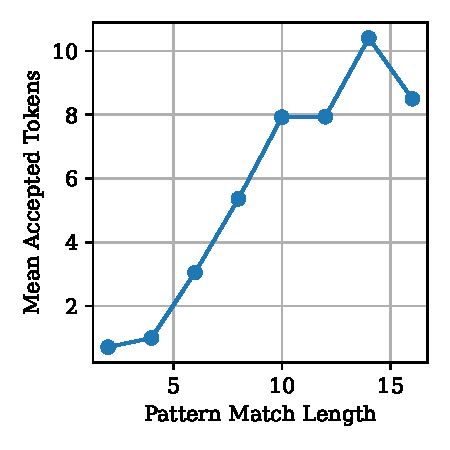
\includegraphics[width=\columnwidth,trim={5 5 5 5},clip]{figures/pattern_vs_accept.pdf}
\caption{Avg accepted tokens vs pattern match length.}
\label{fig:pattern-vs-accept}
\end{subfigure}%
\hspace{1mm}
\begin{subfigure}{0.24\columnwidth}
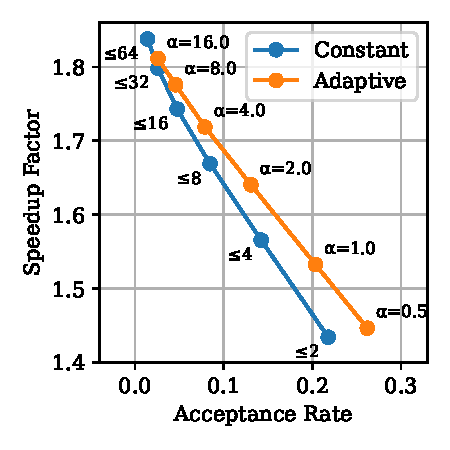
\includegraphics[width=\columnwidth,trim={5 5 5 5},clip]{figures/max_spec_tokens_vs_factor.pdf}
\caption{Using constant vs adaptive \( \texttt{MAX\_SPEC} \).}
\label{fig:constant-vs-adaptive}
\end{subfigure}%}
\caption{(a) the mean number of accepted tokens increases with the length of the pattern match, which motivates \( \texttt{MAX\_SPEC} = \alpha p \). (b) shows that this choice achieves a better trade-off between acceptance rate and speculative speedup.
}
\end{wrapfigure}
%\end{minipage}

\paragraph{Adaptive Speculation Lengths.}

While the procedure above allows SuffixDecoding to cache and quickly speculate long token sequences based on empirical probability estimates, it also needs a mechanism for \emph{adaptively} controlling the number of tokens it speculates. SuffixDecoding achieves this by dynamically adjusting \texttt{MAX\_SPEC}. Low values mean fewer but more likely tokens would be chosen for speculation, while higher values mean more but less likely tokens would be chosen. If too low, then the speedup from speculation can be limited, and if too high, then compute may be wasted on verifying unlikely tokens.

To guide how to adaptively set \texttt{MAX\_SPEC}, we observed that the number of accepted tokens in practice typically increases with longer pattern sequence lengths \( p \) (Fig.~\ref{fig:pattern-vs-accept}). Thus, we define \texttt{MAX\_SPEC} adaptively as
\[
\texttt{MAX\_SPEC}(p) = \alpha p,
\]
where \( \alpha \) is a user-defined max speculation factor. Fig.~\ref{fig:constant-vs-adaptive} shows that setting \texttt{MAX\_SPEC} adaptively according to the pattern length results in a better trade-off between acceptance rate and speculative speedup. In practice, we found that \( \alpha \in [1, 4] \) works well for agentic applications.

\paragraph{Speculation Tree Scoring.}

So far, we have discussed how to obtain a speculation tree given a suffix tree and a pattern length \( p \). However, SuffixDecoding maintains two suffix trees, the global suffix tree and the per-request suffix tree, each with many choices for \( p \). To obtain just a single speculation tree, we build speculation trees for both the global suffix tree and the per-request suffix tree, and for a range of values of \( p \). Then, a single speculation tree is selected according to a scoring function:
\[
\texttt{SCORE}(T_{spec}) = \sum_{N \in T_{spec}} D(N).
\]
Intuitively, if \( D(N) \) estimates the probability that node \( N \) in a speculation tree \( T_{spec} \) would be accepted, then \( \texttt{SCORE}(T_{spec}) \) estimates the expected number of accepted tokens. SuffixDecoding then selects the \( T_{spec} \) with the highest \( \texttt{SCORE} \) as the final speculation tree to be verified.
The end-to-end candidate generation from speculation tree expansion to scoring is described in Alg.~\ref{alg:suffix-decoding}.

\paragraph{\emph{Hybrid} Suffix Speculative Decoding.}

Lastly, we find that \( \texttt{SCORE}(T_{spec}) \) can be used to dynamically decide between using SuffixDecoding or falling back to a model-based speculation method, which is useful for practical scenarios when the workload can be mixed between agentic and more diverse applications. Specifically, for each decoding iteration, we always speculate using SuffixDecoding first. If \( \texttt{SCORE}(T_{spec}) > \tau \), where \( \tau \) is a configurable threshold, then SuffixDecoding's draft tokens are used. Otherwise, we use a fall-back speculation method, such as EAGLE-3~\citep{li2025eagle3scalinginferenceacceleration}. 

As a practical guideline, we find that setting $\tau$ close to the mean accepted tokens of the fallback speculator works well for mixed workloads, while using SuffixDecoding alone ($\tau = 0$) is optimal for highly repetitive agentic tasks. A detailed sensitivity analysis of $\tau$ across different workload types is provided in Appendix~\ref{sec:threshold-sensitivity}. For batched serving scenarios, SuffixDecoding can be integrated with existing batch-level speculation control methods (see Appendix~\ref{sec:batch-speculation}).
